% !TEX program = xelatex
% Cards format — auto-generated from calarts-news.tex by cards-convert.mjs
\documentclass[11pt]{article}

\usepackage{fontspec}
\usepackage{unicode-math}
% Latin Modern by OTF filename (not font name): xelatex on macOS (Core
% Text, no fontconfig) cannot resolve "Latin Modern Roman" by name, which
% silently produced ~4KB broken card PDFs. kpathsea finds the OTFs in
% texmf-dist on both macOS and the oven's Linux xelatex.
\setmainfont{lmroman10-regular.otf}[
  BoldFont=lmroman10-bold.otf,
  ItalicFont=lmroman10-italic.otf,
  BoldItalicFont=lmroman10-bolditalic.otf,
]
\setsansfont{lmsans10-regular.otf}[
  BoldFont=lmsans10-bold.otf,
  ItalicFont=lmsans10-oblique.otf,
  BoldItalicFont=lmsans10-boldoblique.otf,
]
\setmonofont{lmmono10-regular.otf}[Scale=0.88,
  BoldFont=lmmonolt10-bold.otf,
  ItalicFont=lmmono10-italic.otf,
]


\usepackage{graphicx}
\graphicspath{{figures/}{../../papers/arxiv-ac/figures/}}
\usepackage{booktabs}
\usepackage{tabularx}
\usepackage{adjustbox}
\usepackage{ragged2e}
\usepackage{microtype}
\usepackage{natbib}



\makeatletter
\def\input@path{{../}}
\makeatother
\usepackage{ac-paper-cards}


\hypersetup{
  pdftitle={What's New CalArts!?: why the president got booed off the stage --- a letter, with sources},
}

\renewcommand{\acpdfbase}{whats-new-calarts-26-arxiv}
\begin{document}

% ============================================================
% TITLE CARD
% ============================================================
\thispagestyle{empty}
\vspace*{0.05em}
\begin{center}
\href{https://papers.aesthetic.computer}{
\includegraphics[width=0.72\textwidth]{figures/cover}}\par\vspace{0.25em}
{\acbold\fontsize{18pt}{22pt}\selectfont\color{acdark} What's New CalArts!? — A Dossier}\par
\vspace{0.1em}
{\fontsize{9pt}{11pt}\selectfont\color{acpink} why the president got booed off the stage --- a letter, with sources}\par
\vspace{0.2em}
{\scriptsize\color{acgray}\href{https://prompt.ac/@jeffrey}{\color{cyan!70!blue}\textbf{@jeffrey}}\,\textperiodcentered\,Aesthetic{\acdot}Computer\,\textperiodcentered\,ORCID~\href{https://orcid.org/0009-0007-4460-4913}{0009-0007-4460-4913}}\par
\vspace{0.2em}
\rule{0.5\textwidth}{0.5pt}\par
\vspace{0.12em}
\ifacdraft\colorbox{yellow!60}{\small\color{red!80!black}\textbf{\textit{working draft --- not for citation}}}\par
\vspace{0.1em}\fi
{\scriptsize\color{acgray} March 2026 \,\textperiodcentered\, \href{https://github.com/whistlegraph/aesthetic-computer/commit/8fe6526fd}{8fe6526fd}}\par
\end{center}

% ============================================================
% INDEX CARD
% ============================================================
\cardindex

% ============================================================
% ABSTRACT CARD
% ============================================================
\clearpage
\begin{accentcard}
\cardtitle{Abstract}

\noindent Dear Fía and Patrick,\\[0.3em]
ty for sending this --- here's what i know about CalArts so far. you two have
the MFAs; i just have the argument. short clip: the president walks to the
commencement mic, the graduating class boos him off, he freezes for the
better part of a minute, the board chair scolds the kids for booing. that's
it. the long answer to the short \emph{why} is below, from the public record.
one claim runs through it: the boo wasn't an interruption of the institution
--- it \emph{was} the institution. the crit the school actually teaches,
turned for once on the people who run it. a school is a promise about what
its students may become; the boo is that promise auditing its own
administration, out loud, at the ceremony built to keep the gap quiet. with
sources. for you two first. \hfill\textit{---\,@jeffrey}
\end{accentcard}

% ============================================================
% BODY
% ============================================================
\section{The Boo}

On the video, the president of the California Institute of the Arts walks to
the commencement microphone and the graduating class boos until he stops. He
stands frozen for close to a minute. The chair of the board of trustees comes
to the microphone and admonishes the graduates for
booing~\citep{commencement2026video}.

\begin{center}
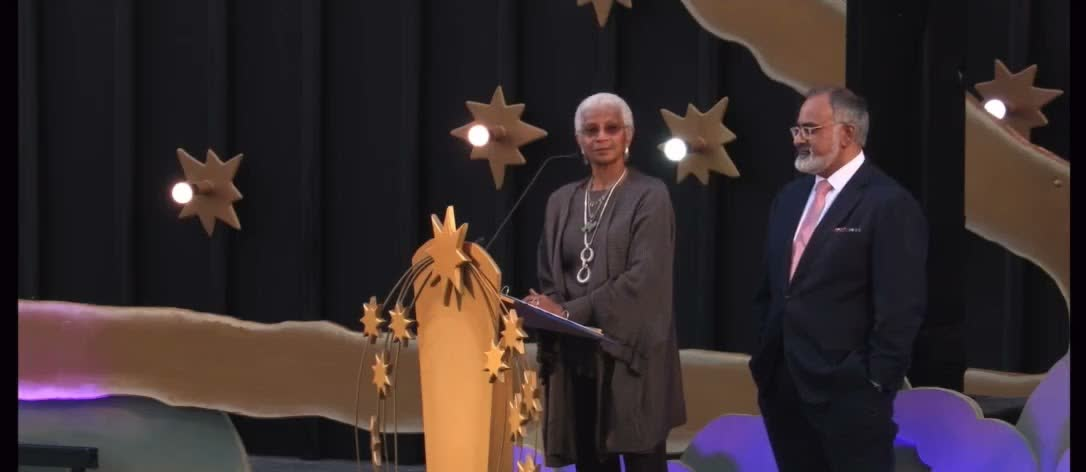
\includegraphics[width=\linewidth]{yt-still}\\[0.15em]
{\footnotesize\color{acgray}\textit{still from the commencement
video~\citep{commencement2026video}: the board chair at the microphone; the
president, beside her, frozen.}}
\end{center}

Begin there, because a commencement is the one rite in which an institution
narrates itself: the address is the school explaining, to the people it has
just finished credentialing, what it believes it has made of them. To boo
that address is not heckling. It is criticism delivered in the institution's
own first language. CalArts teaches the \emph{crit} --- the unscripted,
collective, frequently brutal evaluation of work in a room --- as its central
pedagogy; the crit is, in \citet{elkins2001why}'s account, precisely the part
of an art education that cannot be reduced to method or rubric, and in
\citet{hooks1994teaching}'s, the room in which authority is made to answer for
itself. The graduating class did not drop their training at the door of the
ceremony. They performed it. A crit does not ask \emph{did this meet the
requirements}; it asks \emph{does this deserve to stand}. They asked it of the
presidency, and they answered.

\section{What the School Was For}

Walt Disney chartered CalArts in 1961 by merging the Chouinard Art Institute
with the Los Angeles Conservatory of Music; he died before the Valencia
campus opened in 1971 inside a single long brutalist megastructure by Ladd \&
Kelsey. The founding intent was industrial --- a trained pipeline for the
studio --- but the faculty hired after his death (Kaprow, Baldessari,
Chicago, Schapiro, Paik) turned the building into a laboratory for postwar
American art. \citet{singerman1999art} reads exactly this institution as the
hinge on which the American artist became a \emph{university subject}: the
studio absorbed into the degree, the artist produced by a curriculum.
\citet{deduve1994attitude} names the same shift in its own terms --- the
academy of skill giving way to the post-Bauhaus school of \emph{attitude},
where what is taught is no longer a craft but a stance. CalArts is de Duve's
thesis poured in concrete. Its promise was never a syllabus. It was
proximity, permission, and the dare: put unlike disciplines close enough and
let them contaminate one another, and call the contamination an education.

\section{The Crit Is the Curriculum}

The thing to understand about CalArts --- the thing the budget documents
cannot see --- is that its actual curriculum is not in its catalog. It is in
the room. \citet{elkins2001why} argues that what happens in a good crit is
unteachable in the same sense art is unteachable: it is an oral tradition,
knowledge that exists only in the people who carry it and the time they spend
carrying it together. \citet{freire1970pedagogy} draws the contrast the
school lives by --- the ``banking'' model, in which the institution deposits
value into a passive student, against the dialogic, in which knowledge is
produced between people who can both be wrong. \citet{hooks1994teaching}
insists that this kind of teaching is a practice of freedom or it is nothing,
and \citet{spivak2012aesthetic} that an aesthetic education is, at its limit,
the training of the imagination for solidarity. None of this lives in a line
item. All of it lives in faculty who are present, in governance that is
shared, in a building that forces collision. Which is to say: the school's
real curriculum is exactly the part of it that an administration under
financial pressure will experience as \emph{slack}.

\section{Womanhouse, 1972}

The clearest proof that the promise was real --- and that it was always
students who kept it --- is Womanhouse. In 1971 Judy Chicago and Miriam
Schapiro started the Feminist Art Program; over the winter, twenty-seven
women took a condemned seventeen-room Hollywood mansion and made it into an
installation and performance work that drew roughly ten thousand visitors
between January~30 and February~28, 1972, and was later filmed by Johanna
Demetrakas~\citep{womanhouse2024wiki, calarts_femlib}. It was not assigned. It
was the school's promise executed by its students against the school's own
plan. \citet{harney2013undercommons} give this its sharpest name: the
\emph{undercommons} --- the fugitive intellectual life that the institution
houses, tolerates, and takes credit for, but did not author and cannot
direct. Womanhouse is the undercommons of CalArts made visible for one month.
Every later confrontation on that campus is continuous with it.

\section{The Callout, Pointed Inward (2014)}

The crit has been turned on the administration before. In October 2014, after
an Al Jazeera America report on the school's handling of a sexual-assault
case (a student the coverage called ``Regina''; CalArts found the assailant
responsible; there was no criminal prosecution)~\citep{aljazeera2014regina},
students interrupted a board of trustees meeting on October~15 --- a board
that then included the actor Don Cheadle and the \emph{Los Angeles Times}
publisher Austin Beutner --- and on October~23 walked out of class and
peacefully occupied the administrative offices, hundreds gathering in the
main building~\citep{steinhauer2014walkout, artforum2014walkout}. Faculty
stood with them; the organizer was a graduate student, Cori Redstone; the
demands were structural --- consent education, reformed adjudication,
transparency, a return to shared governance. CalArts was then one of
eighty-five colleges under federal Title~IX investigation.
\citet{fraser2005critique} is the necessary reading here: institutional
critique, she argues, has itself become an institution --- the museum learns
to exhibit its own critique and is strengthened by it; the practice it became
is the one \citet{alberro2009institutional} anthologize. What an institution
\emph{cannot} absorb is the critique that refuses to become an art object: a
walkout has no wall text; a boo cannot be acquired.

\section{The University in Ruins (2017--2026)}

Ravi S.~Rajan became president in 2017, arriving from leadership at SUNY
Purchase~\citep{calarts_rajan_bio}. What the public record shows next reads
like a case study from \citet{readings1996ruins}, whose argument is that the
contemporary university survives by hollowing into an administrative shell
organized around the empty word \emph{excellence} --- a signifier with no
content, which is precisely why anything can be cut in its name. The numbers:
enrollment down roughly twelve percent post-pandemic, from 1{,}532 (2019) to
1{,}353 (2023); tuition above \$60{,}000 for 2025--26; a projected \$15M
structural deficit; about \$5.5M trimmed through spending controls. In April
2024 Rajan told \emph{Inside Higher Ed} the school was ``fiscally sound.'' In
spring 2025 voluntary separations were offered to fifty or sixty people and
thirty-two accepted (twenty-two faculty, ten staff); in July 2025 nine
administrative employees were laid off (five union, four non-union) and twelve
vacant positions cut. Rajan's July~15 letter: ``These are not just abstract
positions---they are roles held by our colleagues, teammates, and friends.''
Faculty and staff had begun organizing in fall 2024; a December 2024 letter
announced intent to organize roughly six hundred workers with the UAW; the
election was held in March 2025 and ratified in
April~\citep{artnewspaper2024union, hyperallergic2025layoffs,
calarts_sustainable2025}. \citet{bousquet2008university} supplies the last
piece: in the financial logic of the contemporary school, faculty are not the
mission --- they are the adjustable variable, the casualizable cost, the
precarious cultural labor \citet{ross2009nice} tracks across the whole
creative economy. Set the readings side by side and the decade resolves: the
administration treated the school's actual curriculum --- present faculty,
shared governance, the density that \emph{is} the teaching --- as the
budget's slack, and narrated the cutting as the only realistic option ---
what \citet{fisher2009capitalist} calls capitalist realism, the management of
decline announced as the absence of any alternative.

\section{Why They Booed}

Now the answer can be stated plainly, and without flattery to anyone.

\citet{bourdieu1977reproduction} established the contradiction that every
serious school lives inside: the institution reproduces the very hierarchies
its pedagogy promises to suspend. CalArts promises proximity, permission, the
dare --- a place where what you are allowed to become is not pre-decided ---
while operating as an institution that must rank, credential, charge sixty
thousand dollars, and balance a deficit --- and \citet{davis2013theses}
locates the art student exactly there: a debt-financed aspirant sold a class
position the market will not honor. The contradiction is not a scandal; it is
constitutive. What changed under the conditions in \S6 is that the
administration stopped pretending the contradiction cost anything. It
narrated ``fiscally sound'' and ``sustainable'' over a decade of cutting the
exact resources that were the school's only real curriculum, and then
scheduled a commencement to narrate, one more time, that the promise had been
kept.

The boo is what \citet{harney2013undercommons}'s undercommons sounds like
when it becomes briefly audible at the institution's own podium. It is
\citet{fraser2005critique}'s un-absorbable remainder: criticism that will not
resolve into an art object, a panel, or a press release, and therefore cannot
be exhibited and neutralized. And it is the school's own pedagogy run
correctly: a crit, convened without permission, asking the question CalArts
taught the room to ask --- \emph{does this deserve to stand} --- of the
people who had spent a decade insisting it did. They were not failing to
graduate. They were giving the institution its final crit, and the
institution, frozen at the microphone for the better part of a minute, had no
answer that the room would accept.

\section{Coda}

So, Fía, Patrick --- here is the short version of the long version. You sent
me forty-five seconds of a man frozen at a microphone while a room refused
him. I went looking for the why and found that the boo was the most CalArts
thing in the entire video. The pedagogy worked. The crit held. The students
did exactly what the school spent two years and an MFA each teaching the two
of you to do: stand behind the judgment, in the room, out loud, with nothing
between you and the work but the question of whether it deserves to exist.
What had stopped working was not the school. It was the administration's
account of the school. I am writing this as a letter and not as a press
release on purpose: a letter has to stand behind itself, in the open, the way
a crit does. That is the only register in which any of this is honest.

\vspace{0.5em}
\noindent\textbf{ORCID:} \href{https://orcid.org/0009-0007-4460-4913}{0009-0007-4460-4913}

\bibliographystyle{plainnat}
\bibliography{references}

\end{document}
